\documentclass[UTF8,12pt]{ctexart}

\usepackage[a4paper,margin=2.2cm]{geometry}
\usepackage{amsmath,amssymb,bm}
\usepackage{graphicx}
\usepackage{booktabs}
\usepackage{array}
\usepackage{caption}
\usepackage{float}
\usepackage{xcolor}
\usepackage{hyperref}
\usepackage{enumitem}
\usepackage{fancyhdr}

\hypersetup{colorlinks=true,linkcolor=blue,urlcolor=blue,citecolor=blue}
\pagestyle{fancy}
\fancyhf{}
\setlength{\headheight}{15pt}
\lhead{Core-Shell V2 EP 验证}
\rhead{\thepage}
\setlist[itemize]{leftmargin=1.5em}
\graphicspath{{figures/}}

\title{\textbf{Core-Shell V2 / PV-Active Shell\\EP 验证结果报告}}
\author{S-H-I-T-ocean / EP-FLUX 工作记录}
\date{2026-09-06}

\begin{document}
\maketitle

\begin{abstract}
本报告整理已经完成的 Core-Shell V2 全生命周期验证结果。核心结论是：当前资料并不支持把涡旋输送强行解释为单一材料涡体积的闭合问题，更合理的框架是
\[
\mathcal{T}_{total}
=
\mathcal{T}_{core}^{trap}
+
\mathcal{T}_{shell}^{stir}
+
\mathcal{T}_{exchange}.
\]
其中 inner core 更接近 Hua/LAVD 近同位的弱速旋转材料核，主要对应 trapping/material coherence；PV-active shell 更接近 PV anomaly、月牙状强速带、热/PV stirring 和 EP 倾斜修正活跃区；exchange layer 用于单独列账 heat/PV/momentum 边界交换。V2 结果显示 PV covariance 更偏 shell，heat covariance 在 coherent 中接近 core/shell 分担、在 upright-like 中更偏 shell，EP 倾斜修正不是小量，且不能只归因于 inner core。
\end{abstract}

\section{运行状态与数据来源}

服务器结果目录为：
\begin{verbatim}
/root/autodl-fs/kuroshiou/EP-FLUX/core_shell_partition_v2
\end{verbatim}
本地镜像目录为：
\begin{verbatim}
G:\TEMP\kuroshiou_ep_core_shell_partition_v2
\end{verbatim}

本轮已经完成 coherent 与 upright\_like 两类 shape 的 V2 分区输出，均使用
\[
\text{radial\_seed axis}+\text{TURN}+\text{thermal\_wind}
\]
口径。服务器日志无 \texttt{Traceback}、\texttt{Killed}、\texttt{MemoryError} 或磁盘不足错误。日志中存在少量 \texttt{Mean of empty slice} 警告，表示部分 \(\tau\)-depth-region 无有效样本或 mask 为空；这些格点应在正式分析中按有效样本数审查。

\section{为什么需要 Core-Shell V2}

早期设想是寻找一个单一材料涡体积，使其同时满足低泄漏、围住弱速旋转核、围住 PV anomaly 核心，并解释热/PV/动量输送。但前期诊断显示，Hua 弱速中心与 LAVD 旋转相干中心通常较接近，而 PV anomaly core 常系统性偏离。这说明运动学旋转核和动力 PV 核不必是同一个对象。

因此 V2 不再要求
\[
PV\ core \subset M_{LAVD},
\]
而是把涡旋结构分为三个物理角色：
\begin{itemize}
  \item \textbf{inner core}：低泄漏、弱速核心连通、Hua/LAVD 近同位，解释 trapping/material coherence。
  \item \textbf{PV-active shell}：高 \(|q'|\)、高 \(|\nabla q'|\)、强剪切或月牙状强速带，解释 heat/PV stirring 和 EP 倾斜修正。
  \item \textbf{exchange layer}：inner core 与 shell 的接触带，单独计算 heat/PV/momentum 边界交换。
\end{itemize}

\begin{figure}[H]
  \centering
  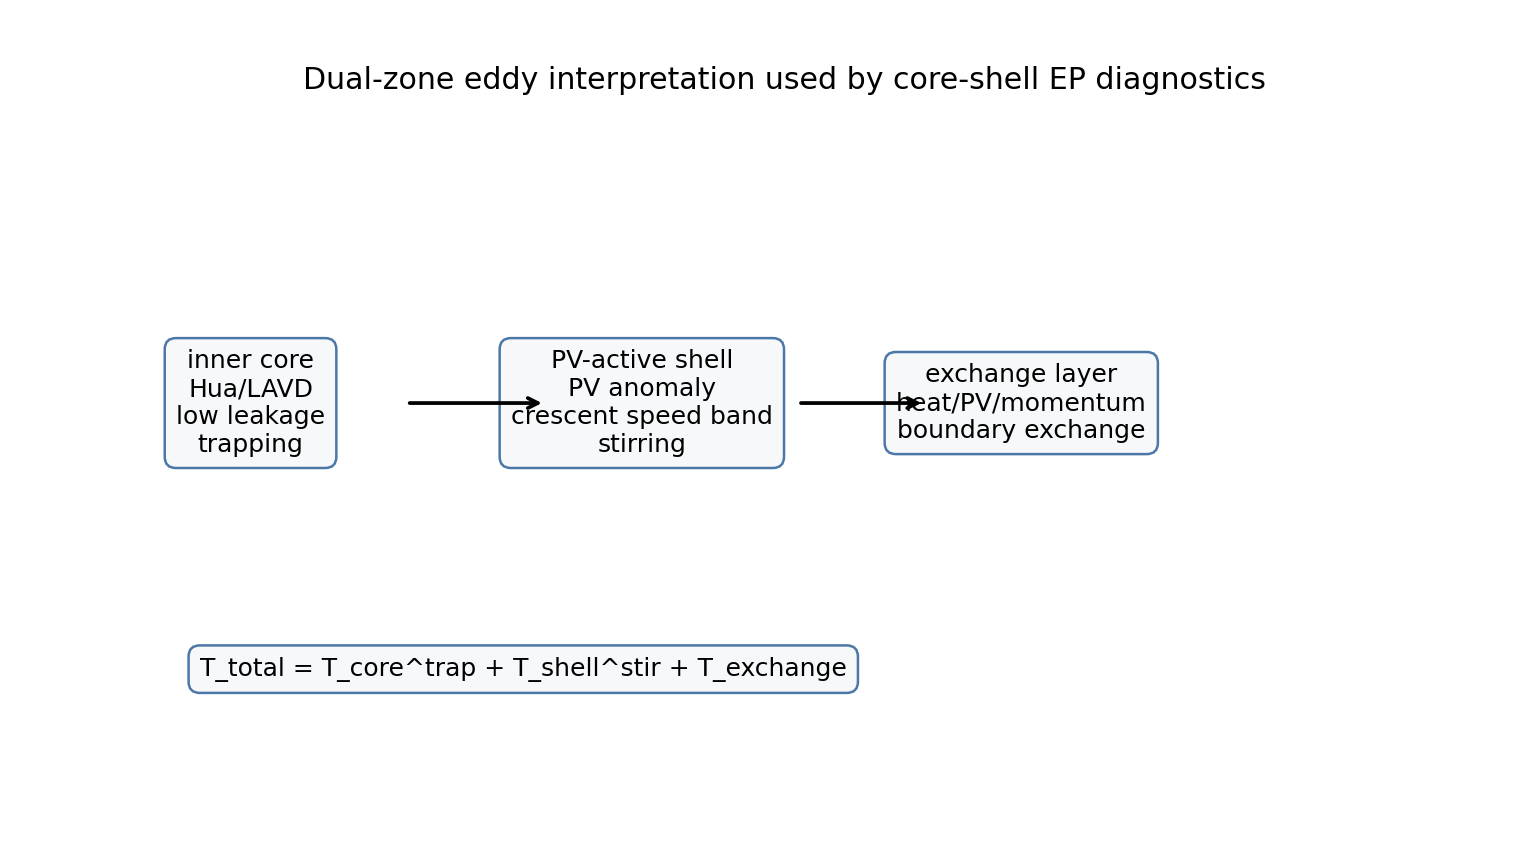
\includegraphics[width=0.78\linewidth]{dual_zone_framework_summary.png}
  \caption{Core-Shell V2 的双区结构示意。inner core 负责 material trapping，PV-active shell 负责 stirring，exchange layer 负责二者之间的边界交换。}
\end{figure}

\section{输送和 EP 公式}

热通量和 PV 通量采用 aggregate-product 口径：
\[
H_M=\rho_0 C_p\langle v'_{rot}\theta'\rangle_M,
\qquad
P_M=\langle v'_{rot}q'\rangle_M.
\]
每个区域 \(M\) 同时保留
\[
\langle vX\rangle_M,\quad
\langle v\rangle_M\langle X\rangle_M,\quad
{\rm cov}_M=\langle vX\rangle_M-\langle v\rangle_M\langle X\rangle_M,
\]
其中 \(X=\theta'\) 或 \(q'\)。这避免了用平均代表涡结构相乘来替代真实协方差输送。

普通垂向 EP flux 写为
\[
F_z^{ordinary}
=
\rho_0 f_0\frac{\langle u_r'b'\rangle}{N^2}.
\]
在倾斜涡旋坐标下，垂向方向不再等同于固定地理 \(z\) 方向，因此记录
\[
F_z^{tilted}
=
F_z^{ordinary}
+
F_z^{tilt\ correction}.
\]
前期全生命周期 EP 结果显示
\[
\frac{|F_z^{tilt\ correction}|}{|F_z^{ordinary}|}
\]
中位数约为 0.47，四分位约为 0.32--0.62，最大可超过 1。这是目前最稳健的正结果：倾斜坐标会显著改写热/浮力相关的垂向 EP flux。

\section{Core-Shell V2 数值结论}

表 \ref{tab:summary} 给出根目录 \texttt{core\_shell\_all\_summary.csv} 的中位数摘要。这里的 heat/PV 贡献指 object-day aggregate covariance 的区域贡献比例。

\begin{table}[H]
\centering
\small
\begin{tabular}{llrrrr}
\toprule
shape & region & heat cov. & PV cov. & tilt corr. & tilt/ordinary \\
\midrule
coherent & inner core & 0.526 & 0.441 & 0.501 & 0.512 \\
coherent & PV shell & 0.475 & 0.559 & 0.498 & 0.382 \\
upright-like & inner core & 0.447 & 0.385 & 0.546 & 0.486 \\
upright-like & PV shell & 0.553 & 0.615 & 0.453 & 0.344 \\
\bottomrule
\end{tabular}
\caption{Core-Shell V2 的主要中位数结果。PV covariance 在两类 shape 中都更偏 shell；heat covariance 在 coherent 中接近 core/shell 分担，在 upright-like 中更偏 shell。}
\label{tab:summary}
\end{table}

\subsection{热通量来自 core 还是 shell}

\begin{figure}[H]
  \centering
  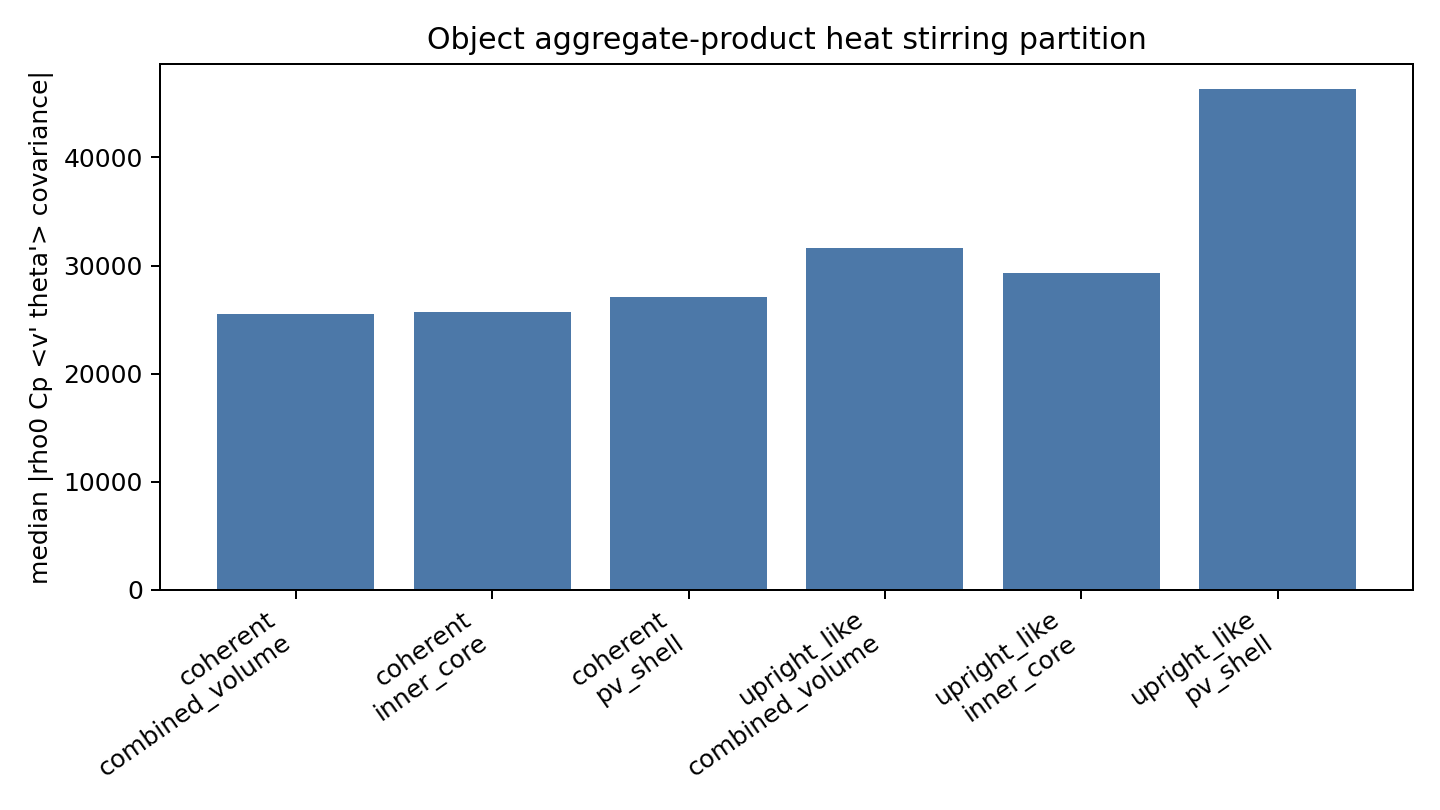
\includegraphics[width=0.88\linewidth]{object_aggregate_heat_core_vs_shell_partition.png}
  \caption{Object-day aggregate-product 热通量分区。coherent 中 heat covariance 接近 core/shell 分担；upright-like 中 shell 贡献更高。}
\end{figure}

这个结果说明热输送不是一个纯粹的材料核问题。对于 coherent，inner core 仍有明显贡献，说明弱速旋转核内部可以承载一部分热异常协方差；但在 upright-like 中，热输送更偏向 shell，说明倾斜和外壳交换会增强热 stirring。

\subsection{PV 通量来自 core 还是 shell}

\begin{figure}[H]
  \centering
  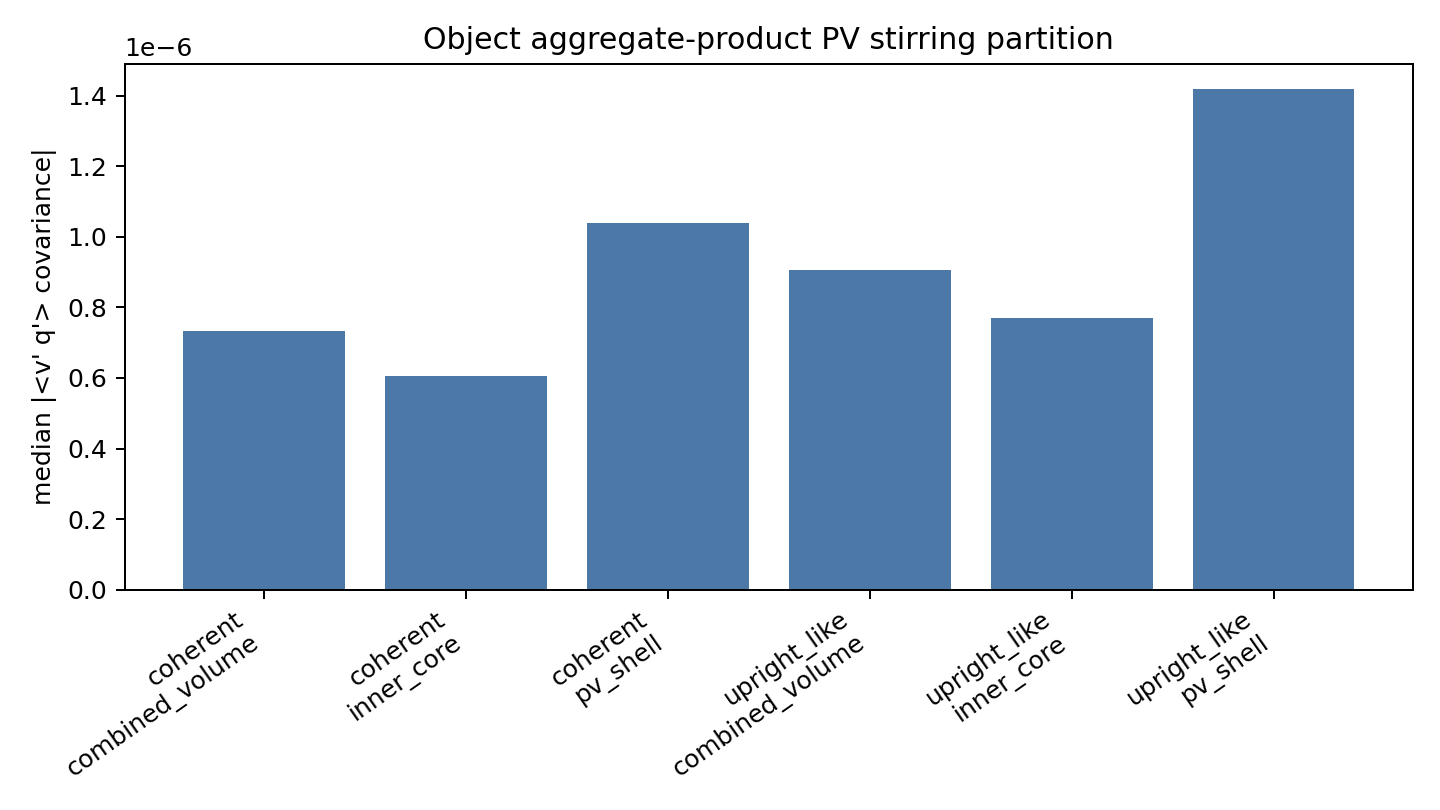
\includegraphics[width=0.88\linewidth]{object_aggregate_pv_core_vs_shell_partition.png}
  \caption{Object-day aggregate-product PV 通量分区。PV covariance 在 coherent 与 upright-like 中均更偏 PV-active shell。}
\end{figure}

PV 的结果比热通量更明确。coherent 的 shell 贡献约为 0.56，upright-like 的 shell 贡献约为 0.61。也就是说，PV stirring 的主体更像外壳或外围强剪切带，而不是低泄漏材料核。这直接支持 ``PV core 不必位于 LAVD core 内部'' 的解释。

\subsection{EP 倾斜修正发生在哪里}

\begin{figure}[H]
  \centering
  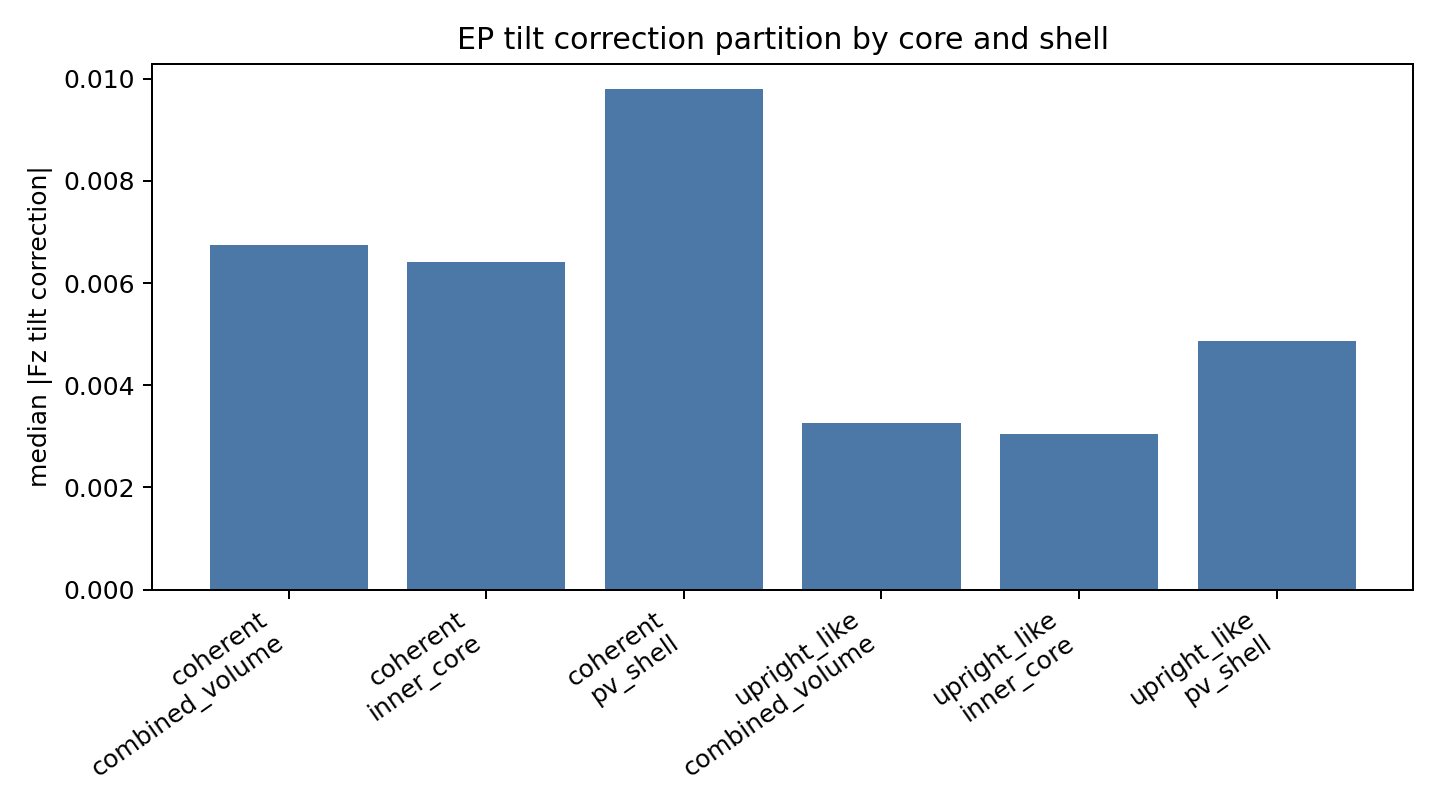
\includegraphics[width=0.88\linewidth]{ep_tilt_correction_core_vs_shell.png}
  \caption{EP 倾斜修正的 core-shell 分区。倾斜修正并非只发生在 inner core；shell 对绝对修正量也有重要贡献。}
\end{figure}

EP 倾斜修正在 coherent 中几乎 core/shell 对半，在 upright-like 中 inner core 略高但 shell 仍不可忽略。这意味着倾斜修正不是一个只依赖中心线的几何小项，而是和整个涡旋截面中的浮力协方差、剪切结构和 shell 交换共同相关。

\subsection{边界交换是否能忽略}

\begin{figure}[H]
  \centering
  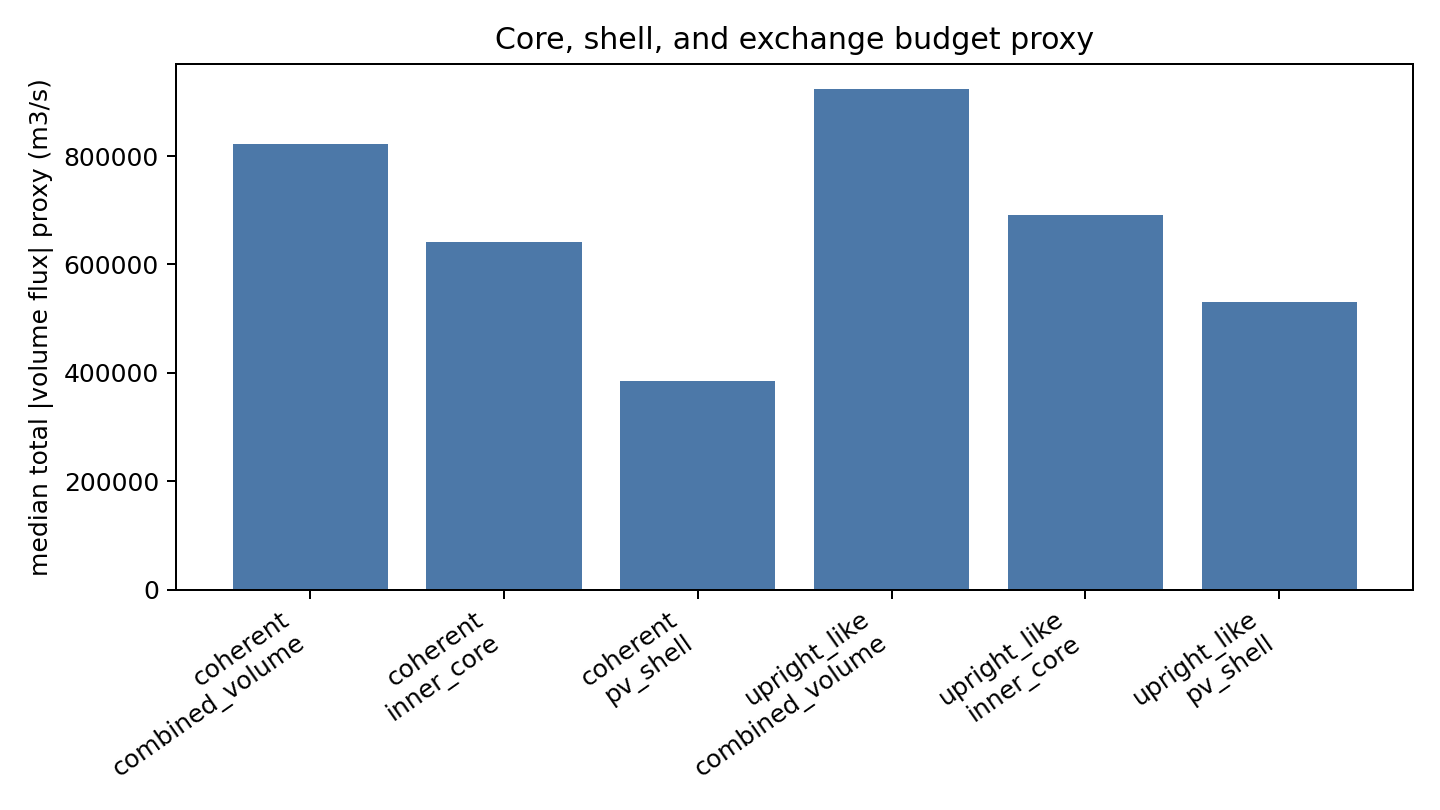
\includegraphics[width=0.88\linewidth]{core_shell_exchange_budget.png}
  \caption{Core-shell exchange budget。边界热、PV、动量交换必须单独列账，不能直接并入内部 EP forcing。}
\end{figure}

\begin{figure}[H]
  \centering
  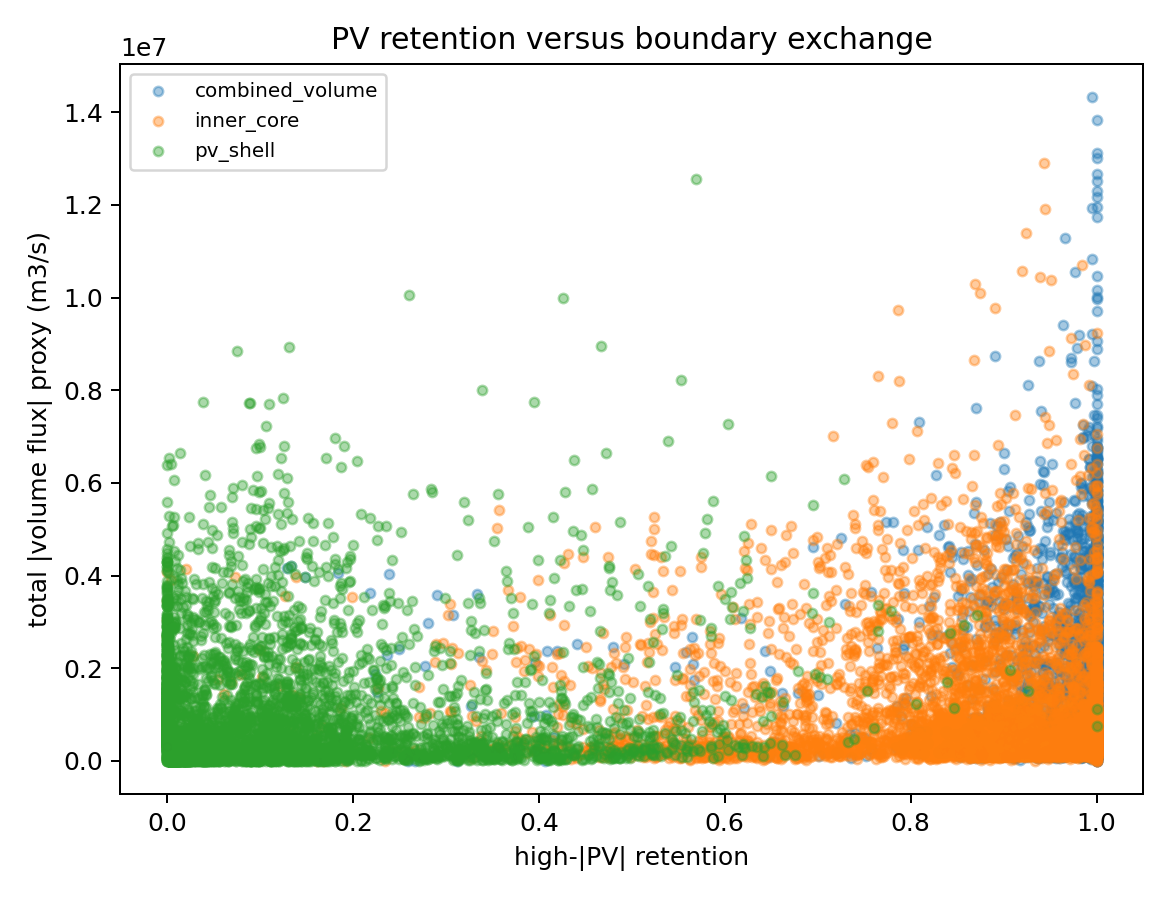
\includegraphics[width=0.88\linewidth]{pv_retention_vs_boundary_exchange.png}
  \caption{PV retention 与 boundary exchange 的关系。若提高 PV retention 的同时 exchange 变大，说明 PV-active shell 和低泄漏 material core 并不完全重合。}
\end{figure}

边界交换不应被当成误差项一笔带过。它正是双区结构中的第三个物理量：inner core 与 PV-active shell 的 exchange layer。后续若要做严格闭合，应该分别列出内部 EP forcing 与边界 heat/PV/momentum exchange，而不是把它们混成一个总通量。

\section{与 thin curved tube 方案的关系}

此前 thin curved tube 方案尝试用 metric、Jacobian、Christoffel 项解释倾斜涡旋中的几何修正。但结果显示该路线不能强解释：\(\epsilon_{curvature}=\kappa r\) 的中位数约为 10--35，远大于小曲率近似要求，且 \texttt{metric\_valid\_fraction\_median=0}。因此当前阶段不应把一阶曲管几何项写成可靠动力 forcing。

这并不否定倾斜修正本身。倾斜修正是由坐标投影和浮力协方差定义直接得到的稳定信号；失效的是把大曲率涡旋塞进 thin curved tube 小曲率展开的几何解释。

\section{理论判定}

Core-Shell V2 目前支持如下判断：
\begin{enumerate}
  \item \textbf{inner core 是 material trapping core}：它更贴近 Hua/LAVD 弱速旋转核，weak-core retention 更高。
  \item \textbf{PV-active shell 是 stirring core}：PV covariance 和高 PV retention 更偏 shell，热 covariance 在 upright-like 中也更偏 shell。
  \item \textbf{exchange layer 是闭合残差的物理来源之一}：boundary exchange 不小，说明严格材料闭合不能只靠低泄漏边界优化。
  \item \textbf{EP 倾斜修正是稳健信号}：修正量约为 ordinary vertical EP flux 的一半量级，不能忽略。
  \item \textbf{完整材料边界强结论尚未完成}：geodesic/LAVD object-level full 没有完整跑完，因此不能声称严格材料体 EP 闭合已经成立。
\end{enumerate}

\section{下一步}

建议按低风险顺序推进：
\begin{enumerate}
  \item 对 object-level 做小样本 geodesic/LAVD + PV-retention 验证，不直接开全量。
  \item 将 heat/PV/momentum boundary exchange 做成独立预算表，确认 shell 是否是主要交换层。
  \item 如果小样本显示 PV-retention 边界能降低 closure residual，再跑 coherent 全量；upright-like 作为对照。
  \item 若 PV retention 提高但 leakage 或 boundary exchange 明显增大，应把结论写成 PV-active shell 与 material core 分离，而不是继续强行寻找单一闭合材料体。
\end{enumerate}

\section{参考文献}

\begin{itemize}
  \item Haller, G. and Beron-Vera, F. J. (2013). Coherent Lagrangian vortices: the black holes of turbulence. \textit{Journal of Fluid Mechanics}, 731, R4. DOI: \href{https://doi.org/10.1017/jfm.2013.391}{10.1017/jfm.2013.391}.
  \item Haller, G. et al. (2016). Defining coherent vortices objectively from the vorticity. \textit{Journal of Fluid Mechanics}, 795, 136--173. DOI: \href{https://doi.org/10.1017/jfm.2016.151}{10.1017/jfm.2016.151}.
  \item Abernathey, R. and Haller, G. (2018). Transport by Lagrangian Vortices in the Eastern Pacific. \textit{Journal of Physical Oceanography}, 48, 667--685. DOI: \href{https://doi.org/10.1175/JPO-D-17-0102.1}{10.1175/JPO-D-17-0102.1}.
  \item Zhang, Z., Wolfe, C. L. P. and Abernathey, R. (2020). Role of Surface-Layer Coherent Eddies in Potential Vorticity Transport. \textit{Fluids}, 5(1), 2. DOI: \href{https://doi.org/10.3390/fluids5010002}{10.3390/fluids5010002}.
  \item Hausmann, U. and Czaja, A. (2012). The observed signature of mesoscale eddies in sea surface temperature and the associated heat transport. \textit{Nature Communications}, 3, 884. DOI: \href{https://doi.org/10.1038/ncomms1595}{10.1038/ncomms1595}.
  \item Dong, C. et al. (2014). Global estimates of oceanic mesoscale eddy heat and salt transports from Argo and altimetry. \textit{Nature Communications}, 5, 3294. DOI: \href{https://doi.org/10.1038/ncomms4294}{10.1038/ncomms4294}.
\end{itemize}

\end{document}
\end{document}
